%%%%%%%%%%%%%%%%%%%%%%%%%%%%%%%%%%%%%%%%%%%%%%%%%%%%%%%%%%%%%%%%%%%%%%%%%%%%%%%
%                         File: osa-revtex4-1.tex                             %
%                        Date: April 15, 2013                                 %
%                                                                             %
%                              BETA VERSION!                                  %
%                   JOSA A, JOSA B, Applied Optics, Optics Letters            %
%                                                                             %
%            This file requires the substyle file osajnl4-1.rtx,              %
%                   running under REVTeX 4.1 and LaTeX 2e                     %
%                                                                             %
%                   USE THE FOLLOWING REVTeX 4-1 OPTIONS:                     %
% \documentclass[osajnl,twocolumn,showpacs,superscriptaddress,10pt]{revtex4-1}%
%                    %% Use 11pt for Applied Optics                           %
%                                                                             %
%               (c) 2013 The Optical Society of America                       %
%                                                                             %
%%%%%%%%%%%%%%%%%%%%%%%%%%%%%%%%%%%%%%%%%%%%%%%%%%%%%%%%%%%%%%%%%%%%%%%%%%%%%%%

\documentclass[osajnl,twocolumn,showpacs,superscriptaddress,10pt]{revtex4-1} %% use 10pt for Applied Optics
%%\documentclass[osajnl,preprint,showpacs,superscriptaddress,12pt]{revtex4-1} %% use 12pt for preprint option
\usepackage{amsmath,amssymb,graphicx,float,enumerate}
% \usepackage[cache=false]{minted}
\usepackage[utf8]{inputenc}
\graphicspath{ {../images/} }

\usepackage[colorlinks = true,
            linkcolor = black,
            urlcolor  = blue,
            citecolor = black,
            anchorcolor = blue]{hyperref}

\usepackage{silence}
\WarningFilter{revtex4-1}{Repair the float}

\begin{document}

\title{Redes y Comunicaciones}

\author{Ulises Jeremias Cornejo Fandos}
\affiliation{13566/7, Licenciatura en Informatica, Facultad de Informatica, UNLP}

\author{Federico Ramón Gasquez}
\affiliation{13598/6, Licenciatura en Informatica, Facultad de Informatica, UNLP}

\author{Lihuel Pablo Amoroso}
\affiliation{13497/2, Analista Programador Universitario, Facultad de Informatica, UNLP}

%%\begin{abstract}
%%\end{abstract}

\maketitle %% required

\onecolumngrid

\section{Ejercicio 1}

\textit{Utilizando topología topologia-IP.imn y dado el bloque IPv6: 2001:db8:1234::/48.}

\section{Ejercicio 2}

\textit{TTL (Adjunte capturas de tráfico para cada uno de los incisos).}

\begin{enumerate}[a)]
    \item \textit{Utilizando el comando \textbf{traceroute6/tracepath6(8)}, realice una
    traza entre el host n8 y n10, tanto utilizando UDP como ICMP.
    ¿Qué diferencias tiene cada método y en qué casos utilizaría cada
    uno?.}


    \item \textit{Realice un ping entre n8 y n5 y determine el valor inicial del
    campo TTL capturando tráfico en la interfaz eth0 del host n8.}

    Para este inciso, se ejecuta en la terminal correspondiente al host n8 un ping entre este host y n5
    utilizando el comando \textit{ping6}. \\

    Capturando el tráfico con el wireshark se busca determinar el valor del campo TTL en
    el header del paquete IPv6. Tras no poder encontrarlo se inspecciona el formato de una
    cabecera IPv6 y concluyendo que dicha información se puede obtener en el header Hop Limit. 
    Leer \href{https://tools.ietf.org/html/rfc2460}{RFC 2460}. \\

    Se puede observar entonces en la figura \ref{image:ttl}, que el valor inicial
    del campo TTL, \textit{Hop Limit en IPv6}, es 64.

    \begin{figure}[H]
        \centering
        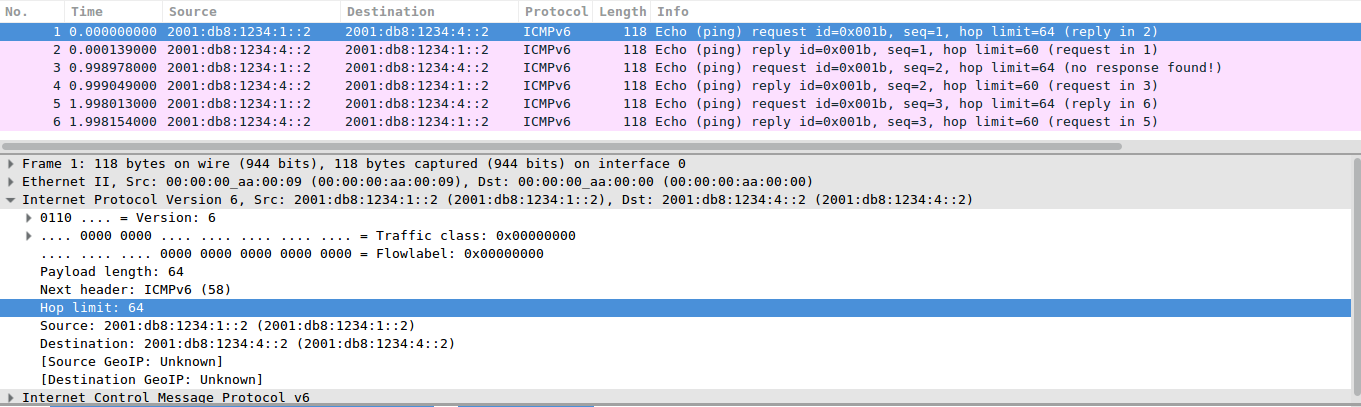
\includegraphics[width=0.95\textwidth]{ttl.png}
        \caption{Captura del tráfico del ping entre n8 y n5 en el que se observa el valor inicial del campo Hop Limit.}
        \label{image:ttl}
    \end{figure}

    \item \textit{A través de la capturas de tráfico, determine en qué momento el
    router decrementa el valor del TTL.}

    

    \item \textit{Utilizando la herramienta para enviar mensajes ICMP con la opción
    -t desde n8 envíe un datagrama a n7 con TTL=1. ¿Qué mensaje recibe? ¿Por qué?}


\end{enumerate}

\end{document}
